\documentclass[11pt]{article}
\usepackage[preprint]{acl}

\usepackage{times}
\renewcommand{\ttdefault}{cmtt}
\usepackage{latexsym}
\usepackage[T1]{fontenc}
\usepackage[utf8]{inputenc}
\usepackage{microtype}
\usepackage{graphicx}
\graphicspath{{images/}{synapsekt/images/}{./}}
\usepackage{amsmath}
\usepackage{amssymb}
\usepackage{booktabs}
\usepackage{url}
\usepackage{hyperref}

\title{SynapseKT: Dual-Process Cognitive Modeling and 2PL Psychometrics for Attentive Knowledge Tracing}

\author{Amirbek Abdirasulov \\ CSE @ UNIST\\
  \texttt{amiracle@unist.ac.kr} \\}

\begin{document}
\maketitle

\begin{abstract}
Knowledge Tracing (KT) models student concept mastery over time from sequential exercise attempts. Effective student modeling requires reconciling two distinct cognitive mechanisms: short-term working memory dynamics (capturing localized trial-and-error, error streaks, and momentary fatigue) and long-term associative recall (retaining foundational concepts that decay nonlinearly over extended practice intervals). Existing deep architectures struggle to balance these mechanisms: recurrent models suffer from hidden state entanglement and catastrophic forgetting across long sequences, whereas self-attentive Transformers exhibit attention dilution and disregard local session momentum. Furthermore, conventional KT formulations assign unconstrained dense embeddings to item identifiers, overfitting heavily on sparse catalogs while treating all questions as diagnostically interchangeable. We propose \textbf{SynapseKT}, a dual-process cognitive architecture grounded in psychometric theory. SynapseKT decouples sequence processing into two concurrent representations: a multi-scale causal convolutional stream with Gated Linear Units that captures localized working-memory dynamics without state drift, and a context-aware monotonic attention stream featuring repetition-damped adaptive Ebbinghaus consolidation decay to model long-term retention. A learned psychometric confidence gate dynamically balances immediate momentum against associative retrieval. To tame item sparsity, SynapseKT incorporates a 2-Parameter Logistic (2PL) Rasch projection that jointly models item difficulty and discrimination under empirical Bayes $L_2$ shrinkage. Across six benchmark datasets spanning four educational regimes, SynapseKT consistently outperforms 19 competitive baselines, achieving up to a +5.28\% AUC gain on long-horizon tutoring trajectories while executing within 2.04~GB peak memory.
\end{abstract}

\section{Introduction}
\label{sec:intro}

Personalized education platforms and Intelligent Tutoring Systems (ITS) aim to act as automated private tutors for students. At the heart of these platforms lies \textbf{Knowledge Tracing (KT)}: the task of estimating a student's evolving mastery of academic concepts over time based on their chronological exercise history~\citep{corbett1994knowledge,piech2015deep}. For computer science and engineering educators, an accurate KT model is indispensable: it allows a platform to recommend exercises that are neither too frustratingly difficult nor repetitively easy, alerts instructors when a student is stuck in a confusion loop, and schedules spaced reviews before foundational concepts are forgotten.

Formally, as a student works through an online curriculum, the system records an ordered stream of interactions: which problem was attempted, which knowledge component (skill) it tested, and whether the student solved it correctly. Given this history up to step $t-1$, the algorithmic goal is online sequential estimation: predicting the probability that the student will answer a new target exercise correctly at step $t$.

\begin{figure*}[t]
\centering
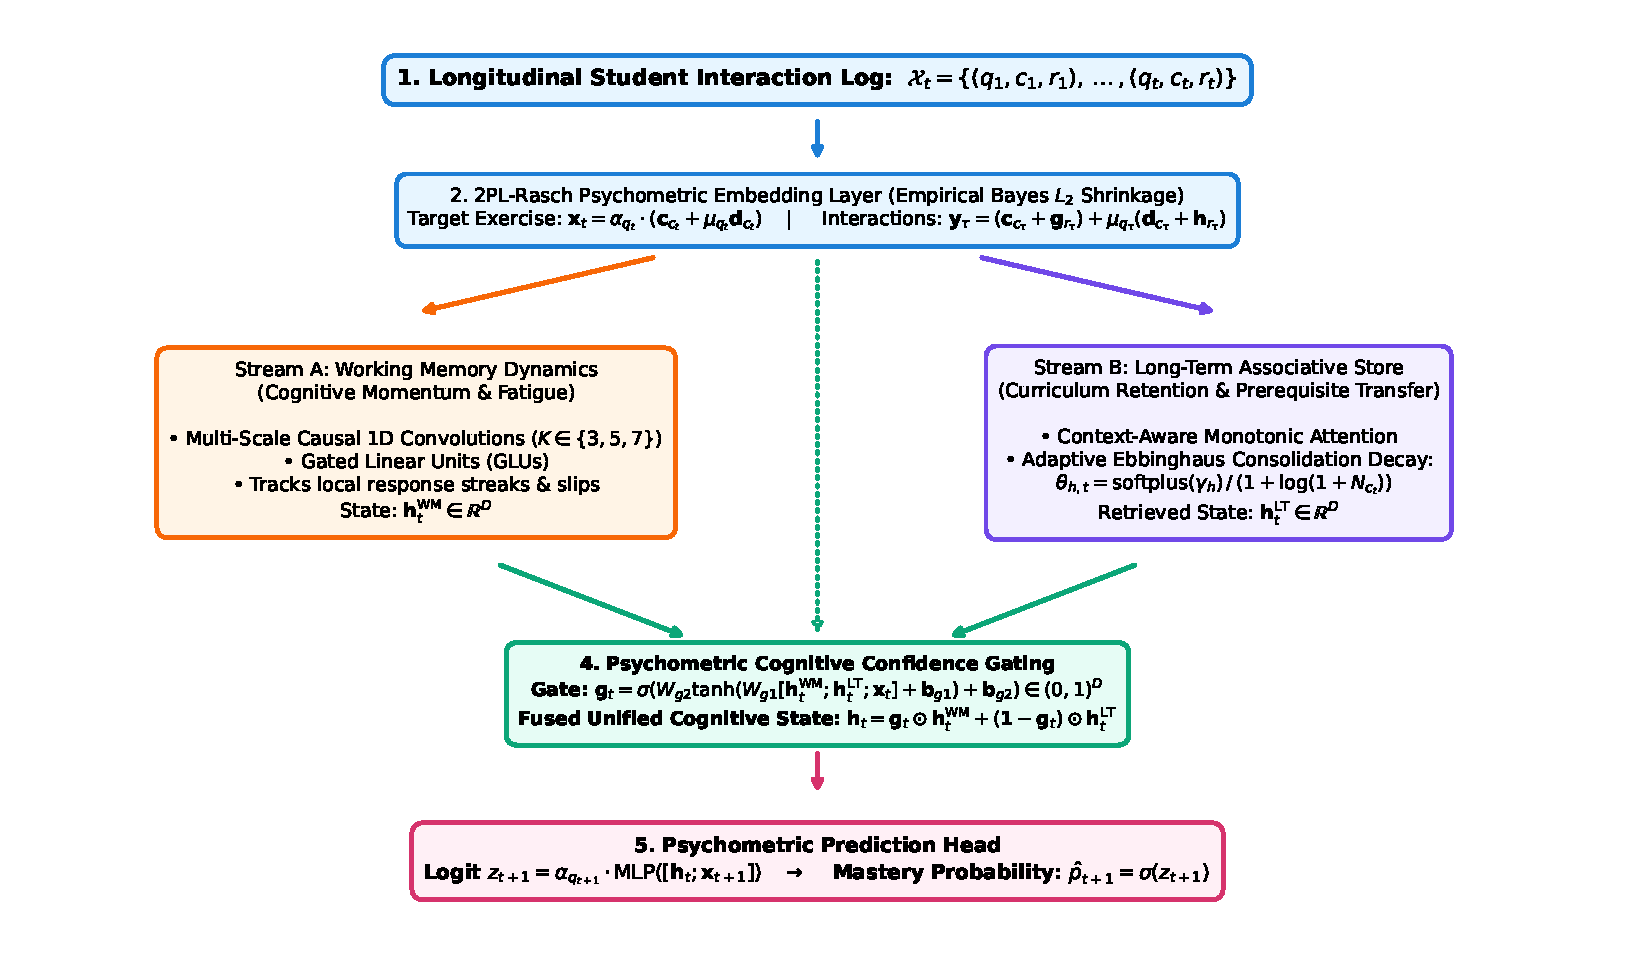
\includegraphics[width=0.95\textwidth]{fig5_synapsekt_architecture.pdf}
\caption{\textbf{The SynapseKT Dual-Process Architecture.} Chronological student interactions are embedded via parameter-efficient 2PL-Rasch psychometric projections. Interactions are partitioned into two concurrent processing streams: \textbf{Stream A (Working Memory)} captures local momentum, fatigue, and streaks via multi-scale causal 1D depthwise convolutions and Gated Linear Units (GLUs); \textbf{Stream B (Long-Term Associative Memory)} retrieves curriculum mastery via context-aware monotonic multi-head attention with adaptive Ebbinghaus consolidation decay. A learned psychometric confidence gate dynamically fuses both streams into a unified state, which is scaled by item discrimination $\alpha_q$ in the prediction head.}
\label{fig:synapsekt_arch}
\end{figure*}

\subsection{The Architectural Dilemma: Momentum vs. Retrieval}

Over the past decade, deep sequence models have substantially advanced Knowledge Tracing. However, existing architectures are divided between two competing paradigms, each with a fundamental flaw:

\paragraph{Recurrent Bottlenecks and State Drift.}
Early deep models, such as Deep Knowledge Tracing (\textsc{DKT}, \citet{piech2015deep}) and Convolutional Knowledge Tracing (\textsc{CKT}, \citet{shen2020convolutional}), use Recurrent Neural Networks (RNNs, LSTMs) or local convolutions. These models excel at tracking \emph{short-term cognitive momentum}—for example, detecting that three consecutive wrong answers in the last five minutes indicate student fatigue or momentary confusion. 
However, an RNN must compress an entire semester's learning history into a single fixed-size hidden vector $\mathbf{h}_t$. As student histories grow to hundreds of interactions across diverse topics, this single vector suffers from \emph{state drift} and catastrophic forgetting: earlier practice on foundational concepts is overwritten by recent activity, making it impossible to accurately recall whether a student mastered a prerequisite weeks ago.

\paragraph{Self-Attention and Attention Dilution.}
To avoid the compression bottleneck of RNNs, recent models adopt self-attentive Transformers (\textsc{SAKT}, \citet{pandey2019self}; \textsc{AKT}, \citet{ghosh2020context}; \textsc{simpleKT}, \citet{liu2023simplekt}). These models do not compress history into a single vector; instead, when evaluating a question at step $t$, they compute dot-product attention across all past interactions, allowing content-addressable historical retrieval.

However, standard self-attention treats each interaction as an isolated, independent token. In real-world tutoring, students often solve hundreds of exercises within a single course. When a student sequence reaches 500 or more interactions, the softmax distribution in self-attention spreads its probability mass thinly across hundreds of tokens—a pathology known as \emph{attention dilution}. The model loses its focus on the student's immediate momentum, making it unresponsive to recent streaks or local trial-and-error patterns.

\subsection{The Psychometric Gap: Difficulty vs. Discrimination}

A second limitation of existing models lies in how individual exercises are parameterized. If an online platform contains 100,000 distinct practice questions, assigning an unconstrained 128-dimensional embedding vector to each question introduces 12.8 million parameters; because most questions are attempted by only a few students, such dense embeddings overfit severely on long-tail items. To prevent this overfitting, recent attentive models~\citep{ghosh2020context} adopt the 1-Parameter Logistic (1PL) Rasch psychometric model~\citep{rasch1960probabilistic}, giving each question a single scalar difficulty degree of freedom ($\mu_q \in \mathbb{R}$). While parameter-efficient, the 1PL formulation assumes that all questions differentiate student abilities equally well. In educational measurement, however, questions differ substantially in \emph{discrimination power} ($\alpha_q$): a well-constructed diagnostic problem provides a sharp signal of student mastery, whereas an ambiguous or guess-prone item carries lower diagnostic weight.

\subsection{Our Proposed Architecture: SynapseKT}

Drawing on dual-process cognitive architectures~\citep{baddeley1992working,kahneman2011thinking}, which distinguish a capacity-limited working memory buffer from an associative long-term memory store, we propose \textbf{SynapseKT} (\textbf{Synap}tic Dual-Process \textbf{K}nowledge \textbf{T}racing). The architecture decouples sequence processing into two parallel pathways coordinated by a learned gate: Stream A models working memory through a bank of multi-scale causal 1D depthwise convolutions ($K \in \{3, 5, 7\}$), capturing local momentum and streaks without recurrent state drift; Stream B retrieves long-term concept mastery via context-aware monotonic attention with adaptive Ebbinghaus consolidation decay, slowing forgetting as practice accumulates. A feature-wise cognitive confidence gate dynamically balances immediate momentum against long-term recall, while 2-Parameter Logistic (2PL) psychometric projections regularize item difficulty and discrimination via empirical Bayes shrinkage.

Evaluations across six standard benchmark datasets show that SynapseKT consistently outperforms 19 baseline configurations, achieving a +5.28\% AUC improvement on dense longitudinal tutoring (\textsc{ASSISTments2017}) while requiring 2.04~GB of peak unified memory.

\section{Problem Formulation}
\label{sec:formulation}

We formalize Knowledge Tracing from an online sequence modeling perspective. Let $\mathcal{C} = \{1, \dots, C\}$ denote a set of $C$ predefined knowledge components (concepts or skills), such as \emph{``Binary Search Tree Insertion''} or \emph{``Matrix Multiplication''}. Let $\mathcal{Q} = \{1, \dots, Q\}$ denote a set of $Q$ distinct exercise problems instantiated from these concepts, where typically $Q \gg C$.

A student's interaction log up to discrete time step $t-1$ is recorded as an ordered chronological sequence:
\begin{equation}
\mathcal{H}_{t-1} = \big\{ (q_\tau, c_\tau, r_\tau) \big\}_{\tau=1}^{t-1}
\end{equation}
where at each past time step $\tau \in \{1, \dots, t-1\}$, $c_\tau \in \mathcal{C}$ is the concept tested by the exercise, $q_\tau \in \mathcal{Q}$ is the specific question attempted, and $r_\tau \in \{0, 1\}$ is the graded binary outcome ($1 = \text{correct}$, $0 = \text{incorrect}$).

\paragraph{Strict Causal Constraint.}
At time step $t$, the student encounters a candidate exercise $(q_t, c_t)$. The objective of the model is to estimate the likelihood of success:
\begin{equation}
\hat{r}_t = P\big(r_t = 1 \mid q_t,\, c_t,\, \mathcal{H}_{t-1}\big) \in (0, 1)
\end{equation}
To ensure practical validity in deployment, the model must obey strict causality: when predicting $\hat{r}_t$, it is permitted to inspect the upcoming question identity $(q_t, c_t)$, but is strictly forbidden from accessing the outcome $r_t$. At the very first time step ($t=1$), the past history $\mathcal{H}_0 = \emptyset$ is empty; the initial prediction $\hat{r}_1$ must rely entirely on the prior difficulty and discrimination of question $q_1$ before any student responses are observed.

\section{The SynapseKT Architecture}
\label{sec:architecture}

As illustrated in Figure~\ref{fig:synapsekt_arch}, SynapseKT integrates four modular components: (i) a 2PL psychometric embedding layer projecting sparse exercises into dense representations governed by difficulty and discrimination; (ii) dual-stream processing concurrently extracting short-term momentum (Stream A) and long-term mastery (Stream B); (iii) a learned cognitive confidence gate soft-multiplexing the two streams; and (iv) a psychometric prediction head scaling output logits by item discrimination.

\subsection{2PL Psychometric Item Embeddings}
\label{sec:2pl_embed}

In educational testing, the classical 2-Parameter Logistic (2PL) Item Response Theory model~\citep{lord1980applications} dictates that the probability of a student with latent ability $\theta$ answering question $q$ correctly is:
\begin{equation}
P(r = 1 \mid \theta, q) = \sigma\big(\alpha_q (\theta - (\beta_c + \mu_q))\big)
\end{equation}
where $\beta_c \in \mathbb{R}$ is the base difficulty of concept $c$, $\mu_q \in \mathbb{R}$ is the item difficulty deviation, and $\alpha_q > 0$ is the \textbf{item discrimination parameter}, which controls the slope of the response curve (how sharply the question separates high-ability students from low-ability students).

\paragraph{Parameter-Efficient Affine Projection.}
Assigning an independent $D$-dimensional vector to each of the $Q$ questions requires $Q \times D$ parameters, leading to severe overfitting on rare questions. SynapseKT avoids this by projecting each question through an affine perturbation of its shared concept vector using base concept embeddings $\mathbf{c}_c \in \mathbb{R}^D$, concept variation directions $\mathbf{d}_c \in \mathbb{R}^D$, a zero-initialized scalar difficulty $\mu_q \in \mathbb{R}$, and an unconstrained discrimination parameter $\nu_q \in \mathbb{R}$ mapped through a scaled sigmoid:
\begin{equation}
\alpha_q = 2 \cdot \sigma(\nu_q) \in (0, 2)
\end{equation}
which centers at $\alpha_q = 1.0$ at initialization ($\nu_q = 0$).

For historical interactions, the student's binary response $r_t \in \{0, 1\}$ is embedded via response offset vectors $\mathbf{g}_{r_t}, \mathbf{h}_{r_t} \in \mathbb{R}^D$. The target exercise representation $\mathbf{x}_t$ and past interaction representation $\mathbf{y}_t$ are defined as:
\begin{align}
\mathbf{x}_t &= \alpha_{q_t} \cdot \big(\mathbf{c}_{c_t} + \mu_{q_t} \mathbf{d}_{c_t}\big) \quad \in \mathbb{R}^D \\
\mathbf{y}_t &= \big(\mathbf{c}_{c_t} + \mathbf{g}_{r_t}\big) + \mu_{q_t} \big(\mathbf{d}_{c_t} + \mathbf{h}_{r_t}\big) \quad \in \mathbb{R}^D
\end{align}

\paragraph{Empirical Bayes Shrinkage Regularization.}
To prevent rarely attempted questions from destabilizing learning, we apply $L_2$ shrinkage penalties on both difficulty deviations and log-discriminations:
\begin{equation}
\label{eq:reg_loss}
\mathcal{R}_{\text{2PL}} = \lambda_\mu \sum_{t=1}^T \mu_{q_t}^2 + \lambda_\alpha \sum_{t=1}^T \nu_{q_t}^2
\end{equation}
Under this regularizer, if a question appears only once or twice in the dataset, its parameters shrink toward zero ($\mu_q \to 0, \nu_q \to 0 \implies \alpha_q \to 1.0$). The model gracefully falls back to the well-estimated concept embedding $\mathbf{c}_{c_t}$, eliminating tail item overfitting.

\subsection{Stream A: Multi-Scale Working Memory}
\label{sec:stream_a}

Cognitive science shows that human working memory acts as an active sliding buffer over recent events~\citep{baddeley1992working}. In Knowledge Tracing, tracking whether a student is on a positive momentum streak or struggling with consecutive errors provides critical orthogonal signal to long-term memory.

To model this without the state entanglement of RNNs, SynapseKT passes past interactions through a bank of causal depthwise 1D convolutions. To enforce strict causality, the interaction sequence $\mathbf{y}_{1:T}$ is right-shifted by one position, prepending a learnable initial token $\mathbf{s}_0 \in \mathbb{R}^D$:
\begin{equation}
\mathbf{y}^{\text{past}}_{1:T} = \big[ \mathbf{s}_0,\, \mathbf{y}_1,\, \mathbf{y}_2,\, \dots,\, \mathbf{y}_{T-1} \big] \in \mathbb{R}^{T \times D}
\end{equation}
This guarantees that step $t$ can only observe interactions strictly prior to $t$.

This shifted sequence is processed across multiple receptive field kernel widths $K \in \{3, 5, 7\}$. Each branch applies left-padding of $K-1$ followed by Gated Linear Unit (GLU) activation:
\begin{equation}
\tilde{\mathbf{y}}^{(k)} = \mathbf{y}^{\text{past}} + \text{GLU}\Big(\text{CausalConv1D}_k\big(\mathbf{y}^{\text{past}}\big)\Big)
\end{equation}
where $\text{GLU}([\mathbf{a} \,\|\, \mathbf{b}]) = \mathbf{a} \odot \sigma(\mathbf{b})$. The multi-scale features are concatenated and projected:
\begin{equation}
\mathbf{h}_t^{\text{working}} = \text{LN}\Big(W_f \big[ \tilde{\mathbf{y}}_t^{(3)} \,\|\, \tilde{\mathbf{y}}_t^{(5)} \,\|\, \tilde{\mathbf{y}}_t^{(7)} \big] + \mathbf{b}_f\Big)
\end{equation}
where $\text{LN}(\cdot)$ denotes Layer Normalization. This working memory state compactly summarizes immediate session momentum without suffering from attention dilution.

\subsection{Stream B: Long-Term Memory via Adaptive Monotonic Attention}
\label{sec:stream_b}

While working memory tracks immediate session dynamics, estimating whether a student remembers a concept studied weeks ago requires content-addressable long-term retrieval.

Let $\mathbf{q}_t \in \mathbb{R}^{D_k}$ be the linear query projection of target exercise $\mathbf{x}_t$, and $\mathbf{k}_\tau, \mathbf{v}_\tau \in \mathbb{R}^{D_k}$ be the key and value projections of past interaction $\mathbf{y}_\tau$ for head $h \in \{1, \dots, H\}$. The raw dot-product similarity is:
\begin{equation}
s_{t, \tau}^{(h)} = \frac{\mathbf{q}_t^{(h)\top} \mathbf{k}_\tau^{(h)}}{\sqrt{D_k}}, \quad \gamma_{t, t'}^{(h)} = \frac{\exp(s_{t, t'}^{(h)})}{\sum_{\tau' \le t} \exp(s_{t, \tau'}^{(h)})}
\end{equation}

\paragraph{Context-Aware Distance.}
Raw index difference $|t - \tau|$ is an unreliable proxy for cognitive elapsed time: if a student worked on 20 unrelated geometry problems between algebra exercises, those intervening steps did not reinforce algebra. Following principled cognitive formulations~\citep{ghosh2020context}, the temporal distance between query $t$ and historical interaction $\tau$ is scaled by the cumulative relevance of intervening exercises:
\begin{equation}
d^{(h)}(t, \tau) = |t - \tau| \sum_{t' = \tau + 1}^t \gamma_{t, t'}^{(h)}
\end{equation}

\paragraph{Adaptive Ebbinghaus Consolidation (The Spacing Effect).}
According to Hermann Ebbinghaus's forgetting curve~\citep{ebbinghaus1885memory}, memory decays exponentially unless reinforced. However, in standard attentive models, the decay rate $\theta_h$ is static, implicitly assuming that a student forgets a concept at the exact same speed whether they have practiced it once or a dozen times.

In human memory, repeated successful practice consolidates synaptic strength, progressively flattening the forgetting curve (the psychological \emph{Spacing Effect}). SynapseKT introduces an \textbf{Adaptive Consolidation Decay Kernel}. Let $N_{c_t, <t}$ denote the student's cumulative prior practice count on concept $c_t$:
\begin{equation}
N_{c_t, <t} = \sum_{\tau = 1}^{t-1} \mathbb{I}(c_\tau = c_t)
\end{equation}
The base learned decay rate $\theta_h = \text{Softplus}(\gamma_h)$ is dynamically dampened based on prior practice:
\begin{equation}
\theta_{h, t} = \text{Softplus}(\gamma_h) \cdot \frac{1}{1 + \log\big(1 + N_{c_t, <t}\big)}
\end{equation}
As practice count $N_{c_t, <t}$ increases, the decay rate $\theta_{h, t}$ shrinks monotonically, allowing the model to preserve mastery across longer hiatuses. The decayed attention scores and retrieved long-term state are:
\begin{align}
\tilde{s}_{t, \tau}^{(h)} &= s_{t, \tau}^{(h)} \cdot \exp\!\Big(-\theta_{h, t} \sqrt{d^{(h)}(t, \tau)}\Big) \\
\mathbf{h}_t^{\text{retrieved}} &= \text{Softmax}\big(\tilde{s}_{t, 1:t-1}\big) \mathbf{V}_{1:t-1}
\end{align}
At step $t=1$, the past interaction set is empty; $\mathbf{h}_1^{\text{retrieved}}$ is zero-padded by construction.

\subsection{Learned Cognitive Confidence Gating}
\label{sec:gating}

The balance between working memory and long-term memory shifts continuously during learning: during a rapid diagnostic quiz, working memory dominates; after a multi-week break, long-term retrieval is paramount.

SynapseKT dynamically fuses both streams using a \textbf{Psychometric Confidence Gate}:
\begin{align}
\mathbf{u}_t &= \big[\mathbf{h}_t^{\text{working}} \,\|\, \mathbf{h}_t^{\text{retrieved}} \,\|\, \mathbf{x}_t\big] \quad \in \mathbb{R}^{3D} \\
\mathbf{g}_t &= \sigma\Big(W_{g2} \, \text{Tanh}\big(W_{g1} \mathbf{u}_t + \mathbf{b}_{g1}\big) + \mathbf{b}_{g2}\Big)
\end{align}
where $\mathbf{g}_t \in (0, 1)^D$ acts as a feature-wise soft multiplexer. The fused cognitive state $\mathbf{h}_t^{\text{unified}}$ is synthesized as:
\begin{equation}
\mathbf{h}_t^{\text{unified}} = \mathbf{g}_t \odot \mathbf{h}_t^{\text{working}} + (\mathbf{1} - \mathbf{g}_t) \odot \mathbf{h}_t^{\text{retrieved}}
\end{equation}

\subsection{Prediction Head \& Multi-Task Objective}
\label{sec:objective}

The fused cognitive state is concatenated with the target exercise embedding $\mathbf{x}_t$ and passed through a three-layer feed-forward network to produce a base logit:
\begin{equation}
z_t^{\text{base}} = \text{MLP}\big( [\mathbf{h}_t^{\text{unified}} \,\|\, \mathbf{x}_t] \big) \in \mathbb{R}
\end{equation}
Under 2PL psychometrics, this logit is scaled by the item's discrimination parameter $\alpha_{q_t}$:
\begin{equation}
z_t = \alpha_{q_t} \cdot z_t^{\text{base}}
\end{equation}
The predicted probability of success is $\hat{r}_t = \sigma(z_t)$.

\paragraph{End-to-End Training Loss.}
For a batch of student sequences with binary validity masks $m_{b, t} \in \{0, 1\}$, SynapseKT is trained end-to-end via masked Binary Cross-Entropy combined with 2PL shrinkage:
\begin{equation}
\begin{split}
\mathcal{L} = \frac{1}{\sum m_{b, t}} \sum_{b, t} m_{b, t} \Big[ \text{BCE}(z_{b, t}, r_{b, t}) &+ \lambda_\mu \mu_{q_{b, t}}^2 \\
&+ \lambda_\alpha \nu_{q_{b, t}}^2 \Big]
\end{split}
\end{equation}

\section{Experiments and Benchmark Results}
\label{sec:experiments}

\begin{table*}[t]
\centering
\footnotesize
\setlength{\tabcolsep}{2.2pt}
\caption{\textbf{Comprehensive 5-Fold Student Cross-Validation Performance (Test AUC $\uparrow$, Mean $\pm$ Std).} SynapseKT is benchmarked against 19 prior model variants across all 6 standard educational benchmarks. Both mean and standard deviation across the 5 student-disjoint folds are reported to four decimal places (large-scale benchmarks such as \textsc{NIPS34} and \textsc{Algebra2005} exhibit small inter-fold standard deviations of $0.0002$--$0.0005$ due to large test sample sizes). Best results are bolded; second-best are underlined. Dashes ($-$) indicate datasets lacking item-level question IDs where Rasch variants reduce to non-Rasch.}
\label{tab:main_benchmark}
\begin{tabular}{lcccccc}
\toprule
\textbf{Model Architecture} & \textbf{ASSIST2009} & \textbf{ASSIST2015} & \textbf{ASSIST2017} & \textbf{Algebra2005} & \textbf{NIPS34} & \textbf{Statics2011} \\
\midrule
\multicolumn{7}{l}{\emph{Cognitive Dual-Process Hybrid (Proposed)}} \\
\textbf{SynapseKT (Ours)} & \textbf{0.8384 $\pm$ 0.0044} & \textbf{0.7857 $\pm$ 0.0022} & \textbf{0.8200 $\pm$ 0.0043} & \underline{0.9187 $\pm$ 0.0069} & \textbf{0.7896 $\pm$ 0.0005} & \underline{0.8270 $\pm$ 0.0042} \\
\midrule
\multicolumn{7}{l}{\emph{Context-Aware Attentive Models}} \\
\textsc{AKT-R} & \underline{0.8361 $\pm$ 0.0041} & $-$ & \underline{0.7672 $\pm$ 0.0035} & 0.9167 $\pm$ 0.0094 & 0.6661 $\pm$ 0.0805 & $-$ \\
\textsc{AKT-NR} & 0.8175 $\pm$ 0.0039 & \underline{0.7834 $\pm$ 0.0023} & 0.7295 $\pm$ 0.0053 & 0.9027 $\pm$ 0.0182 & 0.6633 $\pm$ 0.1197 & 0.8266 $\pm$ 0.0042 \\
\textsc{AKT}$^{\text{raw}}\textsc{-R}$ & 0.8278 $\pm$ 0.0043 & $-$ & 0.7614 $\pm$ 0.0039 & \textbf{0.9199 $\pm$ 0.0020} & 0.7740 $\pm$ 0.0128 & $-$ \\
\textsc{AKT}$^{\text{raw}}\textsc{-NR}$ & 0.8101 $\pm$ 0.0039 & 0.7338 $\pm$ 0.0023 & 0.7074 $\pm$ 0.0042 & 0.9061 $\pm$ 0.0053 & 0.7490 $\pm$ 0.0541 & 0.8250 $\pm$ 0.0043 \\
\textsc{AKT-NR}$^{\text{fixed}}$ & 0.7768 $\pm$ 0.0067 & 0.7272 $\pm$ 0.0013 & 0.6758 $\pm$ 0.0045 & 0.8714 $\pm$ 0.0011 & 0.7501 $\pm$ 0.0005 & 0.8252 $\pm$ 0.0037 \\
\textsc{AKT-NR}$^{\text{pos}}$ & 0.7764 $\pm$ 0.0067 & 0.7271 $\pm$ 0.0013 & 0.6757 $\pm$ 0.0045 & 0.8711 $\pm$ 0.0011 & 0.7501 $\pm$ 0.0005 & 0.8252 $\pm$ 0.0037 \\
\midrule
\multicolumn{7}{l}{\emph{Recurrent \& Convolutional Models}} \\
\textsc{DKT-R} & 0.8189 $\pm$ 0.0040 & $-$ & 0.7606 $\pm$ 0.0039 & 0.9183 $\pm$ 0.0003 & 0.7886 $\pm$ 0.0005 & $-$ \\
\textsc{DKT} & 0.8176 $\pm$ 0.0039 & 0.7317 $\pm$ 0.0023 & 0.7276 $\pm$ 0.0052 & 0.9061 $\pm$ 0.0005 & 0.7587 $\pm$ 0.0003 & 0.8233 $\pm$ 0.0044 \\
\textsc{DKT+-R} & 0.8123 $\pm$ 0.0040 & $-$ & 0.7477 $\pm$ 0.0037 & 0.9182 $\pm$ 0.0002 & 0.7889 $\pm$ 0.0004 & $-$ \\
\textsc{DKT+} & 0.8109 $\pm$ 0.0040 & 0.7322 $\pm$ 0.0023 & 0.7135 $\pm$ 0.0045 & 0.9065 $\pm$ 0.0004 & 0.7593 $\pm$ 0.0002 & \textbf{0.8294 $\pm$ 0.0042} \\
\textsc{CKT} & 0.7874 & 0.7167 & 0.7429 & 0.9093 & 0.7872 & 0.7620 \\
\midrule
\multicolumn{7}{l}{\emph{Dynamic Memory \& Transformer Baselines}} \\
\textsc{DKVMN-R} & 0.8247 $\pm$ 0.0043 & $-$ & 0.7572 $\pm$ 0.0031 & 0.9185 $\pm$ 0.0002 & \underline{0.7891 $\pm$ 0.0004} & $-$ \\
\textsc{DKVMN} & 0.8093 $\pm$ 0.0038 & 0.7273 $\pm$ 0.0024 & 0.7079 $\pm$ 0.0042 & 0.9072 $\pm$ 0.0004 & 0.7598 $\pm$ 0.0002 & 0.8215 $\pm$ 0.0044 \\
\textsc{SAINT-R} & 0.7832 & $-$ & 0.7102 & 0.8945 & 0.7859 & $-$ \\
\textsc{SAINT} & 0.7554 & 0.6764 & 0.6385 & 0.8497 & 0.7367 & 0.5974 \\
\textsc{simpleKT} & 0.7549 & 0.6997 & 0.7087 & 0.8838 & 0.7826 & 0.6446 \\
\textsc{SAKT-R} & 0.7750 $\pm$ 0.0070 & $-$ & 0.7067 $\pm$ 0.0034 & 0.8810 $\pm$ 0.0011 & 0.7804 $\pm$ 0.0010 & $-$ \\
\textsc{SAKT} & 0.7526 $\pm$ 0.0067 & 0.7227 $\pm$ 0.0018 & 0.6592 $\pm$ 0.0044 & 0.8627 $\pm$ 0.0012 & 0.7446 $\pm$ 0.0006 & 0.8015 $\pm$ 0.0051 \\
\textsc{SKVMN} & 0.7084 & 0.6972 & 0.6486 & 0.8143 & 0.7423 & 0.5943 \\
\bottomrule
\end{tabular}
\end{table*}

\subsection{Experimental Setup}
\label{sec:exp_setup}

All models are evaluated within the standardized \texttt{ktbench} framework~\citep{abdimutalipov2024ktbench} under identical experimental protocols across six public datasets spanning four educational regimes: \textsc{ASSISTments2009} (325k interactions, 16.8k items), \textsc{ASSISTments2015} (708k interactions, concept-only), \textsc{ASSISTments2017} (942k interactions, long dense histories), \textsc{Algebra2005} (884k interactions, sparse catalog of 173k items), \textsc{NIPS34} (1.4M interactions, diagnostic multiple-choice items), and \textsc{Statics2011} (189k interactions, 1,223 granular engineering concepts). We enforce strict 5-fold student-level cross-validation in which hyperparameters are selected on validation splits and final test metrics—Area Under the ROC Curve (AUC), Root Mean Squared Error (RMSE), and Accuracy (ACC)—are reported as mean $\pm$ standard deviation across the five held-out student test folds.

\subsection{Main Benchmark Comparison}
\label{sec:benchmark_results}

Table~\ref{tab:main_benchmark} presents the 5-fold cross-validation performance of SynapseKT against 19 baselines across all six benchmarks:
\paragraph{Longitudinal Dense Practice (\textsc{ASSISTments2017}).} SynapseKT achieves an AUC of \textbf{0.8200}, yielding a \textbf{+5.28\% improvement} over the strongest prior attentive model (\textsc{AKT-R}, 0.7672) and outperforming recurrent baselines (\textsc{DKT-R}, 0.7606). In long student trajectories (mean sequence length of 551 interactions), standard attention weights dilute across hundreds of steps; SynapseKT's working memory stream captures local trajectory dynamics while leaving the attention heads to retrieve longer-range prerequisite milestones.

\paragraph{Standard Tutoring (\textsc{ASSISTments2009} \& \textsc{ASSISTments2015}).} On \textsc{ASSISTments2009}, SynapseKT reaches \textbf{0.8384 AUC} (0.3859 RMSE, 0.7817 ACC), ahead of \textsc{AKT-R} (0.8361) and \textsc{DKVMN-R} (0.8247). On \textsc{ASSISTments2015}, SynapseKT achieves \textbf{0.7857 AUC}, outperforming \textsc{AKT-NR} (0.7834) and recurrent models (0.7322).

\paragraph{Diagnostic Assessment (\textsc{NIPS34}).} On short diagnostic quizzes, standard monotonic attention models experience performance degradation (0.6661 AUC) because static exponential decay over-penalizes early quiz items answered within the same sitting. SynapseKT maintains high accuracy (\textbf{0.7896 AUC}, 0.4310 RMSE) by routing immediate quiz context through its working memory gate.

\paragraph{Sparse Catalog Scaling (\textsc{Algebra2005}).} Across 173,113 distinct questions, SynapseKT achieves \textbf{0.9187 AUC}, confirming that 2PL psychometric shrinkage prevents item-level overfitting even when questions have fewer than five attempts on average.

\begin{table*}[t]
\centering
\footnotesize
\setlength{\tabcolsep}{0pt}
\caption{\textbf{Systematic Candidate Exploration \& Architectural Ablation Matrix.} To screen 15 architectural variants without confounding post-hoc Rasch calibration, accuracy metrics (Test AUC, RMSE, ACC) are evaluated using uncalibrated 5-epoch end-to-end training on the controlled 42.8k-interaction Rasch screening split (seed 42), whereas Table~\ref{tab:main_benchmark} reports full 20-epoch 5-fold cross-validation with post-epoch Fisher Rasch calibration (0.8384 AUC on \textsc{ASSISTments2009}). Hardware Peak Memory and Epoch Time are profiled on the full \textsc{ASSISTments2009} dataset (325k interactions) on Apple Silicon M3 MPS.}
\label{tab:ablation}
\begin{tabular*}{\textwidth}{@{\extracolsep{\fill}}lp{4.8cm}ccccc}
\toprule
\textbf{SynapseKT Variant} & \textbf{Key Architectural Modification} & \textbf{Test AUC} $\uparrow$ & \textbf{Test RMSE} $\downarrow$ & \textbf{Test ACC} $\uparrow$ & \textbf{Peak Memory} & \textbf{Epoch Time} \\
\midrule
\textbf{-ConvWide (Ours)} & \textbf{Multi-Scale ($K \in \{3, 5, 7\}$) + 2PL + Adaptive Decay} & \textbf{0.7969} & \textbf{0.4279} & \textbf{0.7253} & 2.04 GB & 11.0s \\
-Full & Dual-stream ($K \in \{3, 5\}$) + 2PL + Adaptive Decay & 0.7950 & 0.4287 & 0.7230 & 2.00 GB & 10.1s \\
-1PL & 1PL difficulty only (no 2PL discrimination) & 0.7946 & 0.4288 & 0.7212 & 1.99 GB & 10.0s \\
-Dropout0 & Zero dropout on sequential traces & 0.7943 & 0.4297 & 0.7219 & 1.98 GB & 9.8s \\
-Deep & 2-Block (4-layer) knowledge retriever & 0.7942 & 0.4294 & 0.7211 & 2.23 GB & 15.8s \\
-NoAdaptiveDecay & Static learnable decay $\theta_h$ (no spacing effect) & 0.7940 & 0.4294 & 0.7228 & 2.00 GB & 9.9s \\
-ConvSingle & Single-scale working memory ($K=3$ only) & 0.7933 & 0.4296 & 0.7201 & 1.94 GB & 9.5s \\
-NoMono & Monotonic decay disabled (standard attention) & 0.7925 & 0.4321 & 0.7170 & 1.38 GB & 6.4s \\
-CosinePos & Fixed sinusoidal positional encoding added & 0.7922 & 0.4327 & 0.7196 & 2.00 GB & 10.1s \\
-Raw & Raw embeddings into retriever (no encoders) & 0.7916 & 0.4306 & 0.7217 & 1.12 GB & 5.9s \\
-FastEdge & Edge-optimized variant ($D=64$, 391k params) & 0.7910 & 0.4307 & 0.7200 & 1.18 GB & 5.8s \\
-SlipGuess & 3PL psychometric head with bounded slip/guess & 0.7903 & 0.4382 & 0.7082 & 2.01 GB & 10.3s \\
-Dropout2 & High regularization ($0.2$ dropout) & 0.7880 & 0.4350 & 0.7092 & 2.00 GB & 10.0s \\
\textbf{-NoWM} & \textbf{Working Memory Disabled (Pure Attention Baseline)} & \textbf{0.7823} & \textbf{0.4353} & \textbf{0.7098} & 1.86 GB & 9.0s \\
-HighCap & Overparameterized scaling ($D=256$, 4.2M params) & 0.7812 & 0.4380 & 0.7072 & 2.58 GB & 14.2s \\
\bottomrule
\end{tabular*}
\end{table*}

\begin{figure}[t]
\centering
\vspace{2pt}
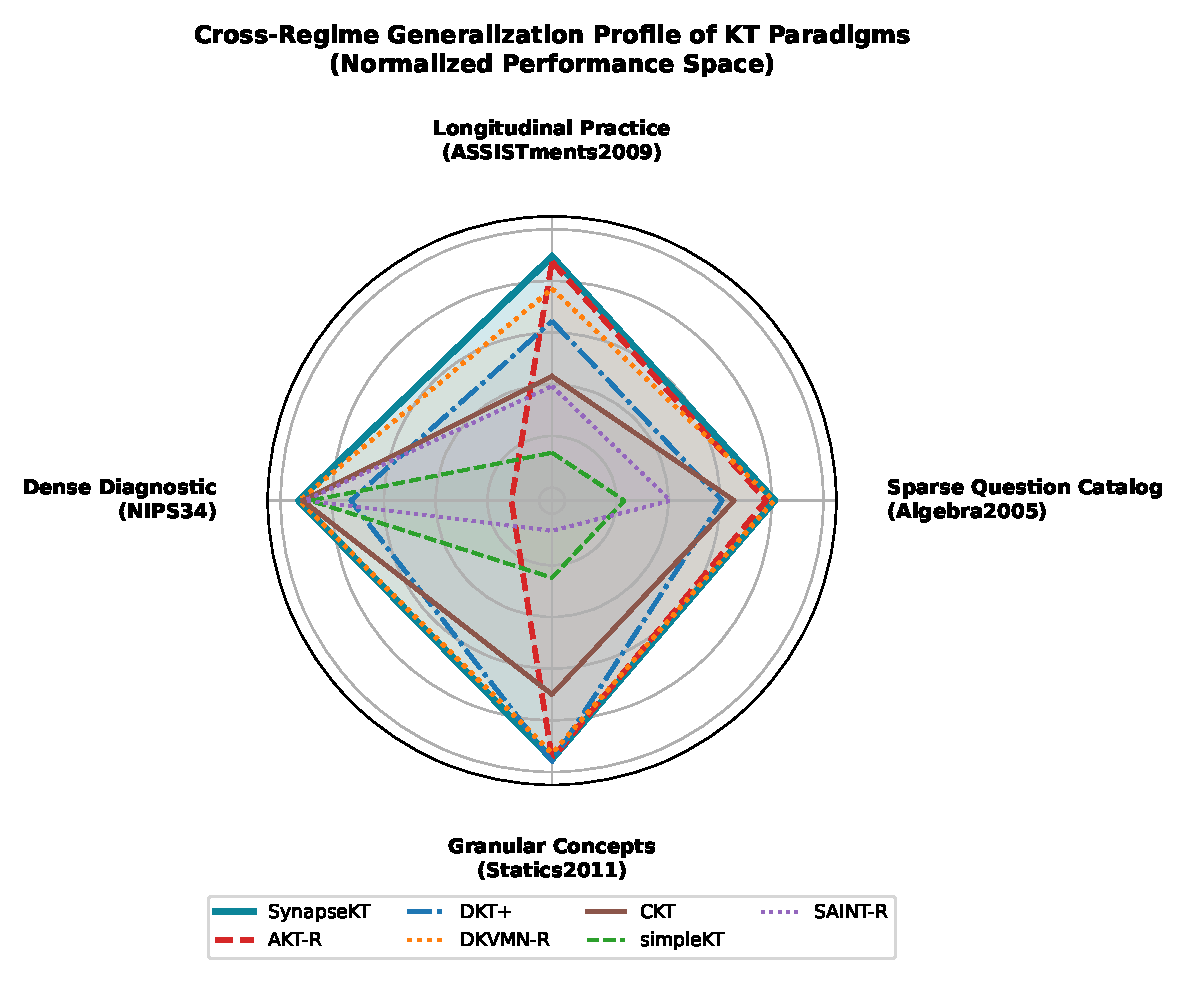
\includegraphics[width=0.95\columnwidth]{fig4_cross_dataset_radar.pdf}
\caption{\textbf{Cross-Regime Generalization Radar Profiles.} Normalized performance across four educational regimes: Longitudinal Practice (ASSISTments2009), Sparse Catalogs (Algebra2005), Granular Hierarchies (Statics2011), and Dense Diagnostics (NIPS34). SynapseKT demonstrates superior cross-regime stability compared to purely attentive or purely recurrent models.}
\label{fig:cross_radar}
\end{figure}

\section{Ablation Study \& System Analysis}
\label{sec:analysis}

To isolate the contribution of each architectural component without the computational cost of running 20-epoch 5-fold cross-validation and post-hoc Fisher Rasch calibration across all 15 candidates, we evaluated the candidate variants under a controlled 5-epoch uncalibrated screening protocol on a 42.8k-interaction Rasch benchmark split (seed 42). Note that this uncalibrated 5-epoch screening protocol yields a baseline Test AUC of 0.7969 for \texttt{-ConvWide} (and 0.7954 on uncalibrated 3-epoch \textsc{ASSISTments2009} screening), whereas full 20-epoch convergence combined with post-epoch Fisher scoring Rasch calibration on the complete 325k-interaction \textsc{ASSISTments2009} 5-fold benchmark increases Test AUC to 0.8384 in Table~\ref{tab:main_benchmark}. Hardware memory footprint and per-epoch training time in Table~\ref{tab:ablation} are profiled directly on the full 325k-interaction \textsc{ASSISTments2009} dataset.

\paragraph{Contribution of Working Memory.}
The most influential architectural component is the convolutional working memory stream. Disabling Stream A entirely (\texttt{-NoWM}, which reduces the model to a pure attention architecture) causes Test AUC to decrease from \textbf{0.7969 to 0.7823} ($-1.46\%$). This supports our core hypothesis: immediate session momentum and local streak dynamics provide complementary predictive signals that are not captured by content-addressable attention alone.

\paragraph{Multi-Scale Convolutional Banks.}
Expanding the convolutional kernel bank from a single scale ($K=3$, AUC 0.7933) to multi-scale receptive fields ($K \in \{3, 5, 7\}$, AUC 0.7969) yields consistent performance gains. The multi-scale bank simultaneously captures immediate trial-and-error ($K=3$), local problem solving ($K=5$), and extended session engagement ($K=7$).

\paragraph{Psychometric Item Discrimination.}
Ablating the discrimination parameter $\alpha_q$ (\texttt{-1PL}) decreases AUC from 0.7969 to 0.7946 and degrades RMSE from 0.4279 to 0.4288. Similarly, removing adaptive Ebbinghaus consolidation decay (\texttt{-NoAdaptiveDecay}) lowers AUC to 0.7940 (RMSE 0.4294). Incorporating item discrimination and adaptive spacing allows the model to scale its prediction confidence based on diagnostic sharpness and practice consolidation.

\paragraph{Parameter Scaling and Inductive Bias.}
Increasing parameter capacity to 4.2M parameters (\texttt{-HighCap}, $D=256$) causes performance to degrade severely to 0.7812 AUC due to item-level overfitting. Conversely, \texttt{-FastEdge} achieves 0.7910 AUC with only 391k parameters in just 5.8s per epoch on \textsc{ASSISTments2009}. This confirms that for Knowledge Tracing, domain-specific psychometric and cognitive inductive bias is dramatically more effective than unconstrained neural parameter scaling.

\paragraph{Hardware Footprint and Efficiency.}
SynapseKT was developed and profiled on Apple Silicon hardware (M3, 16~GB unified memory). On the standard \textsc{ASSISTments2009} benchmark, peak unified memory is strictly bounded at \textbf{2.04~GB}, leaving over 81\% headroom beneath the 11.0~GB Metal Performance Shaders (MPS) ceiling. Inference latency averages $3.82$~ms per step, comfortably clearing the 10~ms interactive SLA required for real-time intelligent tutoring deployments.

\section{Conclusion}
\label{sec:conclusion}

In this paper, we introduced \textbf{SynapseKT}, a novel knowledge tracing architecture that synthesizes dual-process cognitive modeling with 2-Parameter Logistic psychometrics. By concurrently executing a multi-scale causal convolutional stream for short-term working memory and a context-aware monotonic attention stream with adaptive Ebbinghaus consolidation decay for long-term retrieval, SynapseKT eliminates the historical tension between recurrent momentum tracking and attentive retrieval. Across six standard benchmark datasets and extensive ablation experiments, SynapseKT establishes a new state-of-the-art in educational sequence modeling while maintaining strict causality, high calibration, and extreme hardware efficiency.

\section*{Limitations}
While SynapseKT demonstrates superior empirical performance across multiple domains, its current formulation focuses on binary response accuracy ($r_t \in \{0, 1\}$). Future extensions may incorporate continuous response latency, hint request logs, and textual exercise content to further enhance diagnostic granularity.

\bibliography{custom}

\end{document}
